\section{Material \& Methods}

\subsection{Data collection}
I collected data on body size of fossil testudinids from the Miocene until recent times. The body size data set includes 26 fossil genera, comprising over 100 fossil species. The majority of the data was obtained from the primary literature (Table \ref{tab:DataFossil}). To find relevant publications, I relied mostly on the references listed in the FosFarBase \citep{Bohme2003b}, the Paleobiology Database (http://paleobiodb.org), and the review on fossil turtles and tortoises by \cite{rhodin2015turtles}.
Furthermore, the FosFarBase provided fossil occurrences of testudinids all over the world, including their exact localities and age (Table \ref{TabS2}\todo{put table only on CD?}), which were used to get an overview over the availability of body size data. The FosFarBase (http://www.wahre-staerke.com/, last accessed 23.03.2017) contained 769 testudinid occurrences between the Eocene (33.9 - 56 mya) and the Holocene from 647 localities (Fig. \ref{fig:mapOc}). Of those, 641 occurrences from 534 localities were of relevant age (Miocene to Holocene). The final body size data set, however, includes 376 data records from 193 localities, of which 106 localities are present in the FosFarBase.


%__________________________________________________________________
 \begin{figure}[htbp]
 	\centering
 	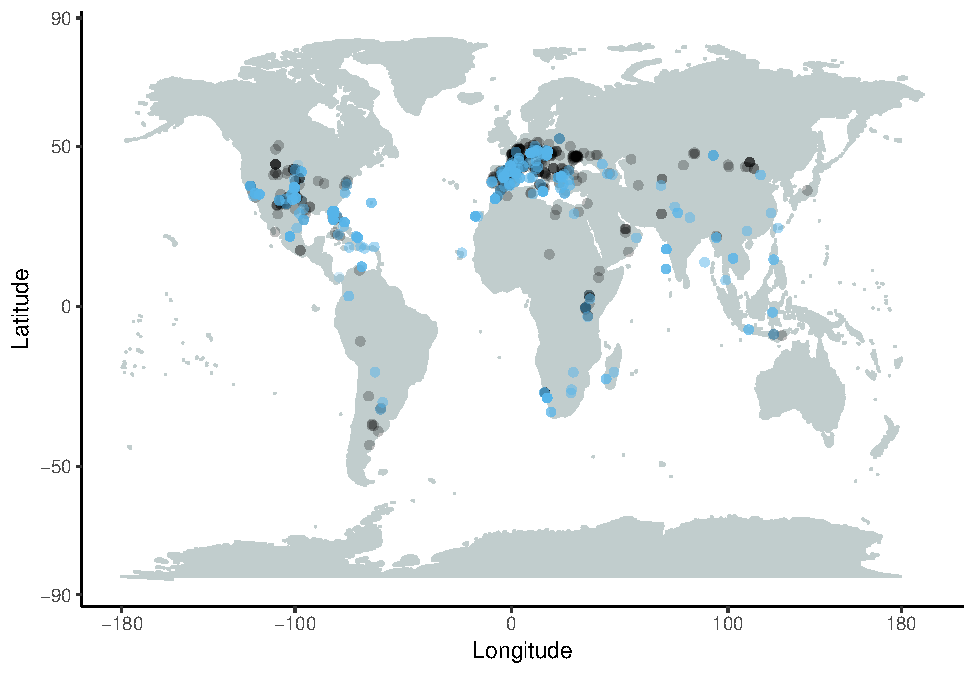
\includegraphics[width=\textwidth]{MA_JJ_files/figure-latex/MapFossilOccurrences-1.pdf}
 	\caption[Map: fossil occurences]{Map displaying all fossil occurrences of testudinids from the Eocene to the Holocene according to the FosFarBase, with
 		color indicating whether body size data was available (blue) or not (black).}
 	\label{fig:mapOc}
 \end{figure}

For extant testudinid taxa, I measured dry material (n = 67) from the collection of the Museum für Naturkunde zu Berlin (MFN) with an accuracy of the first decimal (unless stated otherwise) using calipers. In addition, body size data (n = 173) from the literature was included (Table \ref{tab:DataExtant}).

\subsection{Body size estimation}
Body size is reported as straight carapace length (SCL) in mm. Where SCL for fossil taxa was not available from the primary literature, it was estimated (n = 254) either from plastron length (PL) or appendicular elements (Table \ref{tab:DataFossil}). For carapace length estimations based on plastron length, the measurements from the MFN collection material were used to calculate the ratio between SCL and PL. Since the SC/PL ratio was similar for all species (SCL/PL between 0.95 - 1.47), a single general ratio (SCL/PL = 1.1) was calculated for all testudinids and hence used for the SCL estimations unless stated otherwise (Table \ref{tab:DataFossil}). For estimations based on femora and humeri, ratios based on data provided by \cite{Hutterer1998} and \cite{Franz2001a}, respectively, were used. A number of publications did not state measurements but instead provided scaled figures of the fossil remains, from which either SCL directly or PL, humeri, or femora lengths for estimating SCL could be measured.

%TO DO: check Franz \& Quitmyer, 2005 again!! (CL regression)



\subsection{Analyses}
All subsequent analyses were performed with R 3.4.1 \citep{RCoreTeam2017}, including the packages dplyr \citep{Wickham2017} to prepare the data for the analysis and ggplot2 \citep{Wickham2009} to create figures. The R package vegan \citep{Oksanen2017} was used to create individual-based (?) accumulation curves \todo{check correct term!}, which show the increase in individuals, species or genera per sampling unit and are therefore used to determine if sampling is sufficient or not in terms of covering diversity and richness \citep{Thompson2002}. Most commonly these accumulation curves are conducted on individual or species level, but they can also be applied on higher taxa like families and genera \citep{Gotelli2011, Gotelli2001}. The accumulation curves also give information about species richness, relative abundance and diversity \citep{Thompson2002}. Typically a species accumulation curve shows a steep initial slope followed by gradual plateuing until converging to an asymptote, when the maximum number of species has been reached. However, this shape can be affected in several ways, e. g. when a lot of rare species opposed to only a few abundant species are present or if sampling is conducted on a large geographical scale, the inflection point may be lower and the following slope towards the asymptote may be rather long or an asymptote may not be reached at all \citep{Gotelli2011, Gotelli2001}. \todo{figure necessary?}
Since the data set in this study relies on literature, references were used as a sampling unit (x-axis). %and reach a maximum, when no new species/genera are added. 
Sampling accumulation curves were created on species as well as genus level, since genera of fossil testudinids are relatively well resolved by now whereas determination on the species level is still obscure in some cases, because fossil species are frequently based on single individuals that are often fragmentary as well \citep{Brattstrom1961, DeLapparentdeBroin2001}. Since genera were better sampled than species (Fig. \ref{fig:SACGen}, \ref{fig:SACall} (a) - (b)), all subsequent analysis were performed on the generic level.
Additional sampling accumulation curves for the continents were created (Fig. \ref{fig:SACall} (c) -  (i)), to check if subsequent analyses could be applied to these subgroups. 
% read Species Accumulation Curve papers + Catalinas paper!
% REWRITE

%SACs: tell us if sampling is sufficient (covers all species) and can be used to estimate species richness
%randomization smooths out 

% Gotelli and Colwell, 2011:
% First, the number of individuals that must be sampled to reach an asymptote can often be prohibitively large (Chao et al. 2009). The problem is most severe in the tropics, where species diversity is high and most species are rare.
%%In other words, biodiversity samples, even very extensive ones, often fall short of revealing the complete species richness for an assemblage, representing some unspecified milestone along a slowly rising species accumulation curve with an unknown destination. A second reason that the species accumulation curve cannot be used to directly determine species richness is that, in field sampling, ecologists almost never collect random individuals in sequence. Instead, individual plants or mobile animals are often recorded from transects or points counts, or individual organisms are collected in pitfall and bait traps, sweep samples, nets, plankton tows, water, soil, and leaf litter samples, and other taxon-specific sampling units that capture multiple individuals (Southwood & Henderson 2000).  --> why sample-based SACs are created!!

%Once this asymptote is reached, the species accumulation curve is flat and additional sampling will not yield any additional species. Why should the species accumulation curve have an asymptote? On large geographical scales, it does not: larger areas accumulate species at a constant or even an increasing rate because expanded sampling incorporates diverse habitat types that support distinctive species assemblages (see Chapter 20). As a consequence, the species accumulation curve continues to increase, and will not reach a final asymptote until it approaches the total area of the biosphere.

%Biodiversity sampling is a labour-intensive activity, and sampling is often not sufficient to detect all or even most of the species present in an assemblage.
%Species richness counts are highly sensitive to the number of individuals sampled, and to the number, size, and spatial arrangement of samples.
%Sensitivity to sampling effort cannot be accounted for by scaling species richness as a ratio of species counts to individuals, samples, or any other measure of effort.
%Sample-based and individual-based rarefaction methods allow for the meaningful comparison of diversity samples based on equivalent numbers of individuals and samples.

%% Gotelli and Colwell, 2001:
%In Fig. 1, note that the two sample-based curves lie below the two individual-based curves. The reason for this nearly universal pattern is that sample-based protocols aggregate individuals, within each sample, that are nearby in space or consecutive in time. Any spatial or temporal autocorrelation (patchiness or heterogeneity) in taxon occurrence will cause taxa to occur nonrandomly among samples. Consequently, when a group of samples is pooled, fewer species will be represented by those individuals than by an equal number of individuals censused randomly and independently in the same habitat.
%Raw species richness counts or higher taxon counts can be validly compared only when taxon accumulation curves have reached a clear asymptote. For invertebrate and microbial assemblages everywhere and for many taxa in tropical habitats, such asymptotes may never be reached (e.g. Stork 1991; Wolda et al. 1998; Fisher 1999; Anderson & Ashe 2000; Novotny & Basset 2000). Fortunately, if one or more accumulation curves fail to reach an asymptote, the curves themselves may often be compared, after appropriate scaling.

%%documentation vegan package:  All these methods are based on sampling sites without replacement. In contrast, the method = "rarefaction" finds the expected species richness and its standard deviation by sampling individuals instead of sites. It achieves this by applying function rarefy with number of individuals corresponding to average number of individuals per site.
%specpool normally uses basic Chao equation, but when there are no doubletons (a2=0) it switches to bias-corrected version. In that case the Chao equation simplifies to S_0 + (N-1)/N * a1*(a1-1)/2.


%%%
%cite Lapparent de Broin 2000b: Geochelone is no longer to be used --> introduce Testudo/Geochelone issue (or in introduction?)

\subsubsection{Descriptive statistics}
Normalized histograms with density curves and boxplots of the entire data set and several subgroups (fossil vs. modern, insular vs. continental) were created to explore the structure of the data set. Descriptive statistics like mean \todo{SD needed??}, median, variance, and with the R package moments \citep{Komsta2015} skewness and kurtosis were calculated (Table \ref{tab:stats}) for the raw data and log-transformed data. While mean, median and variance describe the location and distribution of a data set, skewness and kurtosis are referred to as 'shape statistics'. They give information about symmetry (skewness) and the weight of the tails compared to the rest of the distribution, i. e. outliers will results in a higher kurtosis. However, the accuracy and suitability of these shape statistics has been debated, since sample size, extreme values and homogeinity of the data impact their results and uncertainties are higher than mean, median and the like \citep{McNeese2016, Bai2005}. Especially for small sample sizes, the histograms should provide more appropriate information about the structure of the data set than skewness and kurtosis \citep{McNeese2016}.

The Wilcoxon Rank Sum Test (unpaired data) was used to test for differences in body size between modern and fossil taxa as well as between insular and continental taxa. To be able to compare different subgroups, a subsample (1000 repeats) of the respective larger subgroup was taken to compare equal sample sizes.
The Kruskal-Wallis test was used to test for differences between more than two subsamples, e. g. body size per time bin and body size per continent.
As post-hoc test, the Wilcoxon Rank Sum Test was used and a Bonferroni correction applied  to adjust p-avlues.


%- only used samples > 23.000 mya?!

\subsubsection{Body size trends over time}
To investigate trends in body size over time, the R package paleoTS \citep{Hunt2015a} was used. Data were split into time bins according to stratigraphic stages (Table \ref{tab:bins}, Fig. \ref{fig:bins}), although the two lower stages of the Miocene were considered as one time bin, because the last bin otherwise would have contained only 2 data records. To prevent sampling bias and because sampling accumulation curves showed that the genus level was better sampled than species level, the mean SCL per genus was calculated before the timescale analysis. The paleoTS plots display the mean trait over time and can be fitted to different evolutionary models: stasis, where the trait mean fluctuates around a steady mean (no change), generalized random walk (GRW), where changes in trait mean increases or decreases over time (directional change) or unbiased random walk (URW), where trait means change over time but not in a way where they accumulate and move in a specific direction (non-directional change). Model fits are based on maximum-likelihood estimation and model support is reported as Akaike Information Criterion (AICc), with the lowest values indication the best suited model. Additionally, Akaike weights are reported, which give the proportional support for each model. paleoTS plots and model-fitting was performed for the entire data set, continental and insular genera. The same approach was repeated for European and Eurasian genera for all data, as well as continental and insular genera separately.

\todo{explain evolutionary models/fits and AICc etc.}




%__________________________________________________________________
\begin{figure}[htbp]
	\centering
	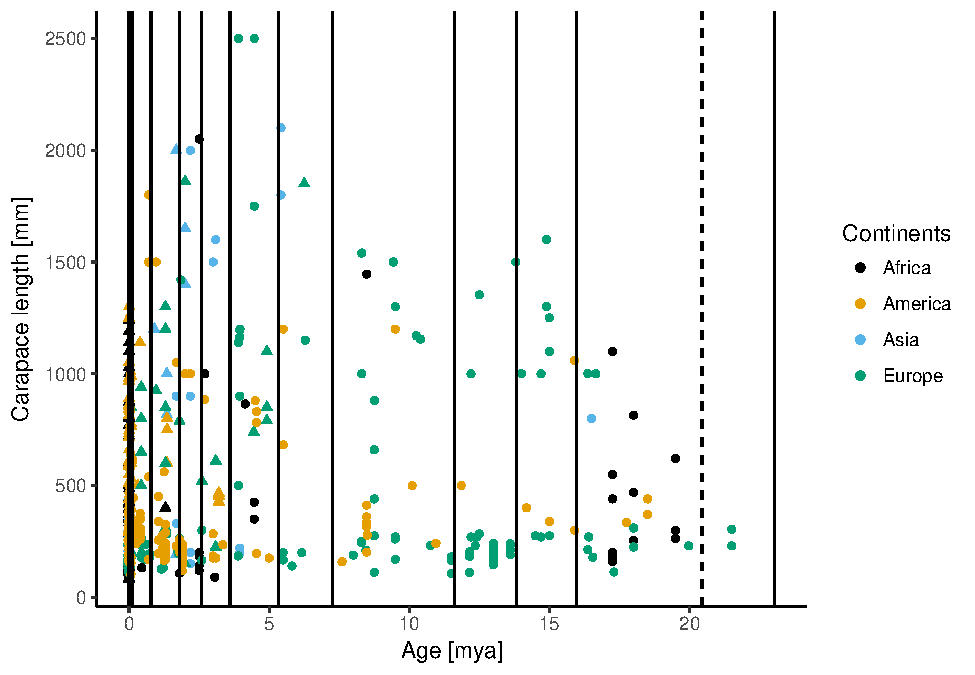
\includegraphics[width=0.8\textwidth]{MA_JJ_files/figure-latex/overviewData-1.pdf}
	\caption[Carapace length over time]{Scatterplot of carapace length over time, indicating insular
		(triangle) and continental (circles) and colour indicating continents.
		Lines indicate stratigraphic stages which were used as time bins, the
		dashed line is the border between the two stages of the Lower Miocene,
		which were consideres as one time bin.}
	\label{fig:bins}
\end{figure}


\begin{landscape}\label{data}
	\begin{longtable}[]{@{}lllcccc@{}}
		\caption[Sample sizes per time bins]{Time ranges, mean age per bin, corresponding stratigraphic stages and epochs, and respective sample sizes (on individual, species and genus level).)}
		\label{tab:bins}\tabularnewline
		\toprule
		Age Range [mya] & Mean Age [mya] & Stages & Epochs & n (Individuals) & n (Species) & n (Genera)\tabularnewline
		\midrule
		\endhead
		0 - 0.0117 & 0.00585 & Modern & Modern & 254 & 66 & 18\tabularnewline
		0.0117 - 0.126 & 0.06885 & Upper Pleistocene & Upper Pleistocene & 50
		& 18 & 8\tabularnewline
		0.126 - 0.781 & 0.45350 & Middle Pleistocene & Middle Pleistocene & 53
		& 13 & 7\tabularnewline
		0.781 - 1.81 & 1.29350 & Lower Pleistocene & Lower Pleistocene & 57 &
		27 & 12\tabularnewline
		1.81 - 2.59 & 2.19700 & Gelasian & Lower Pleistocene & 33 & 15 &
		9\tabularnewline
		2.59 - 3.6 & 3.09400 & Piacencian & Upper Pliocene & 24 & 15 &
		10\tabularnewline
		3.6 - 5.33 & 4.46600 & Zanclean & Lower Pliocene & 31 & 17 &
		8\tabularnewline
		5.33 - 7.25 & 6.28900 & Messinian & Upper Miocene & 12 & 9 &
		6\tabularnewline
		7.25 - 11.6 & 9.42700 & Tortonian & Upper Miocene & 46 & 20 &
		9\tabularnewline
		11.6 - 13.8 & 12.71400 & Serravallian & Middle Miocene & 27 & 8 &
		6\tabularnewline
		13.8 - 16 & 14.89500 & Langhian & Middle Miocene & 18 & 14 &
		9\tabularnewline
		16 - 23 & 19.50000 & Burdigalian/Aquitanian & Lower Miocene & 31 & 15 & 9\tabularnewline
		\bottomrule
	\end{longtable}
\end{landscape}






\FloatBarrier
